\documentclass[letterpaper, 10 pt, conference]{ieeeconf} 

\usepackage{graphicx}

\overrideIEEEmargins

\title{\LARGE \bf
Skull Stripping Axial FLAIR MRIs\\ of the Brain using Machine Learning
}

\author{Vipul Kashyap and Jerry Li \\ %
Computer Science 188 \\
UCLA - Spring 2017 
}

\begin{document}

\maketitle
\thispagestyle{empty}
\pagestyle{empty}

%%%%%%%%%%%%%%%%%%%%%%%%%%%%%%%%%%%%%%%%%%%%%%%%%%%%%%%%%%%%%%%%%%%%%%%%%%%%%%%%
\begin{abstract}
In this project our goal was to segment brain tissue in axial FLAIR MRIs using machine learning. We were successfully able to accomplish this by training a random forest of trees classifier to determine with high accuracy and speed whether a pixel is part of the brain tissue or not. The classifier was given the value of the pixel, the location of the pixel, and the values of nearby pixels. Using preprocessing we were able to ensure that the algorithm can handle moderate contrast differences between images. Using a two phased post processing approach we were able to attain better skull stripping bit masks. Overall, we attained a very good mean Dice score of 97.02. We hope to increase this in the future by using a larger set of training data.
\end{abstract}
%%%%%%%%%%%%%%%%%%%%%%%%%%%%%%%%%%%%%%%%%%%%%%%%%%%%%%%%%%%%%%%%%%%%%%%%%%%%%%%%

\section{INTRODUCTION}
Skull stripping refers to the process of isolating the brain from other structures in a medical image of the brain. This usually involves the removal of the skull and any other non-brain tissue from the image, such as the dura and scalp. It is often done as a preprocessing step as it is improves the speed and accuracy of many brain image analysis/processing algorithms while also decreasing algorithm complexity \textsuperscript{[1]}. \par
Our goal was to segment the brain tissue in MR images with reasonably high accuracy and speed. Since traditional techniques require tuning of several numerical parameters depending on the dataset to achieve the reasonable results, we used machine learning to develop a more effective and easier to use tool. Unlike most other skull stripping techniques we also removed the ventricles. We focused on axial FLAIR MRIs of the brain. \par
A paper by Kleesiek et al had already applied a deep learning architecture to this problem (attaining a mean dice score of 95.19 for clinical data)\textsuperscript{[2]} and so we decided to explore a different approach. Our algorithm used each pixel's location and value as well as the values of neighboring pixels to determine whether the pixel was part of brain tissue. We optimized multiple parameters and applied various techniques to ensure that our tool was flexible enough to work on different MR images regardless of the noise/contrast differences in the images and would provide the best results. \par
We manually skull stripped anonymized MRI data provided by the University of California, Los Angeles to create our training and testing data. The tool was written in Python and relies on various Python libraries such as Google's SciKit-Learn and PyDicom.

\section{METHODS AND CONSIDERATIONS}

\subsection{Data Collection}
The University of California, Los Angeles provided us with MRI data. In order to process this data to create our training and testing data, first anonymized all images to remove all personally identifiable information and then manually skull stripped the images using OsiriX. In OsiriX, we created ROIs for the ventricles and the brain. We used a mixture of the threshold, confidence, and neighborhood methods to creating ROIs and applied different parameters to generate the best fitting ROIs for each feature. We used OsiriX's "Set pixel values" feature to set the pixels inside the ventricles and outside the brain to a value of 0 and set the pixels in the middle of the ventricle and brain ROIs to 1000, giving us the bit masks (which served as our ground truth). Note, we chose to use OsiriX instead of other easier and more automated methods to creating masking images since it gave us finer control over generating the images. All images and masks were 16 bit DICOM files, with heights of 256 pixels and varying widths (all less than 400 pixels).

\subsection{Feature Selection}
There are three major aspects which were considered in determining whether or not a pixel can be considered part of the brain tissue:
\subsubsection{Value of the Pixel}
In general, we see in the FLAIR MRIs that parts of the image which are not brain tissue are dark, meaning they have lower pixel values. This means we can use pixel values as a factor in predicting whether or not a pixel is part of the brain.
\subsubsection{Location of the Pixel}
Pixels very far away from the center of the MRIs and pixels in the very center (ventricles) are unlikely to be part of the brains. We can use X and Y distances from the center as a predictor. Note, we do not use the pixel's euclidean distance from the center because the brain is elongated and not symmetric so just the distance is not a good predictor. Furthermore, since the images have differing widths, just the coordinates do not function as good predictors. A pixel with X value of 5 may be part of the brain in an image with a very small margin, but will be very unlikely to be part of the brain in an image with a large margin. Using the distance from the center helps us avoid this problem.
\subsubsection{Value of Neighboring Pixels}
Patterns among neighboring pixels can help us determine whether the pixel is part of the brain tissue. For example, the texture of the skull tissue or the cerebrospinal fluid in the ventricles can suggest that the pixel is not part of brain, the presence of two edges in the neighboring pixel can suggest that the pixel is between the brain and the skull, etc. An important aspect of this is the number of pixels we consider. After testing several different values, we found that analyzing the surrounding 11x11 grid of pixels gave us the best results. Very small grid sizes resulted in large number of false positives while larger grid sizes gave us results which were difficult to generalize to non-training images. 

\subsection{Estimator Selection}
Our goal was to predict whether or not each pixel was part of brain tissue. This meant that we would be using either classification or clustering estimators. Since we wanted to use our labeled data, classification estimators made the most sense. Furthermore, we were expecting large amounts of data points and so we wanted something scalable. This lead us to using a gradient decent classifier, however our results were terrible and we achieved an ~45\% accuracy among our training data. It was clear that this would not work. Thus, we switched to a Support Vector Machine based classifier. Although it would be a little less scalable, it would provide us with better results . Although this improved our training score to ~60\%, this was still unacceptable. \par
From here we tried the KNeighbors Classifier. This classifier gave us fantastic results with about ~98+\% accuracy, however as the training data grew, the classifier's run time grew exponentially (going above ~1+ minute per image to train, ~4 minutes per image to process, and giving us a 700+MB classifier "pickle" - all with 8 threads running). This classifier was not scalable. \par
Finally, we used ensemble classifiers which provided us with scalable yet good results. The forests of randomized trees classifier allowed us to attain results similar to the KNeighbors classifier (97+\% accuracy on the training data) but was much faster (~10 seconds per image to train, 30 seconds per image to process, 15 MB classifier). 

\subsection{Generalizing For MRI Variation}
We wanted to ensure that our trained model would be robust against mild variation between MRIs. We considered the following attributes of MRIs: 
\subsubsection{Differences in contrast}
We noticed that some MRIs were brighter than others. Some had backgrounds which were almost gray. This was resulting in a model that was not being trained correctly and was unable to tackle variations in MRIs. We were able solve this problem by preprocessing all the images. We centered all images to the mean and scaled them to unit variance before training on them or predicting their skull stripped result.
\subsubsection{Differences in size}
Since our images had varying widths, we were unable to just use the X and Y positions of the pixels and instead used the distance of the pixels from the center. We also considered using ratio's of the X and Y positions versus the width and the heights, but we quickly saw that this did not make sense since the images were not scaled differently, only the margins were different.
\subsubsection{Differences in noise}
We also wanted to account for noise in the images. We did this by adding a preprocessing step of slightly blurring the images. Unfortunately, this resulted in worse results and so it was undone. We also tried downscaling images to half their size, processing them, and then upscaling them again. We hoped that this would allow the model to consider a larger region of the image for each pixel, however it only resulted in lower resolution and less accurate results. Although we were unable to find an effective way to fight noise differences between images, it was not a big concern as it did not have a significant impact on our overall results.

\subsection{Post Processing and Optimizations}
Although our results were quite good (dice score of 91.90), we wanted to see how we could postprocess the bit masks to get even better results. We tried two approaches:
\subsubsection{Neighbor Analysis}
We loop through each pixel in the image and if more than 84\% (tested out different values) of the pixels in the 5x5 grid around it are of a specific type (0 or 1), we change its type to match the majority. This would allow us to fill in small holes in the image. We also tried doing  multiple passes of this but that resulted in too many false positives. Neighbor Analysis yielded a slightly increased mean dice score of 92.08.
\subsubsection{Two Phased Training}
We have two phases. The first phase is the same as our original apporach and trains the algorithm normally. This allows it to create the skull stripping bit masks from MRIs. The second phase uses a different training set to generate bit masks using the learning from phase 1 and then train the same algorithm to take these bit masks and make them more like the ground truth. This two phased approach gave us a better results with a mean Dice score of 94.82.

When we combined both approaches we attained a mean Dice score of 97.01. It was clear that the two-phased approach was the way to go.

We also enabled multiprocessing in our training and batch skull stripping functions for faster results. We gained a linear decrease in time spent training/processing depending on the number of cores the machine has.

\begin{figure}
\centering
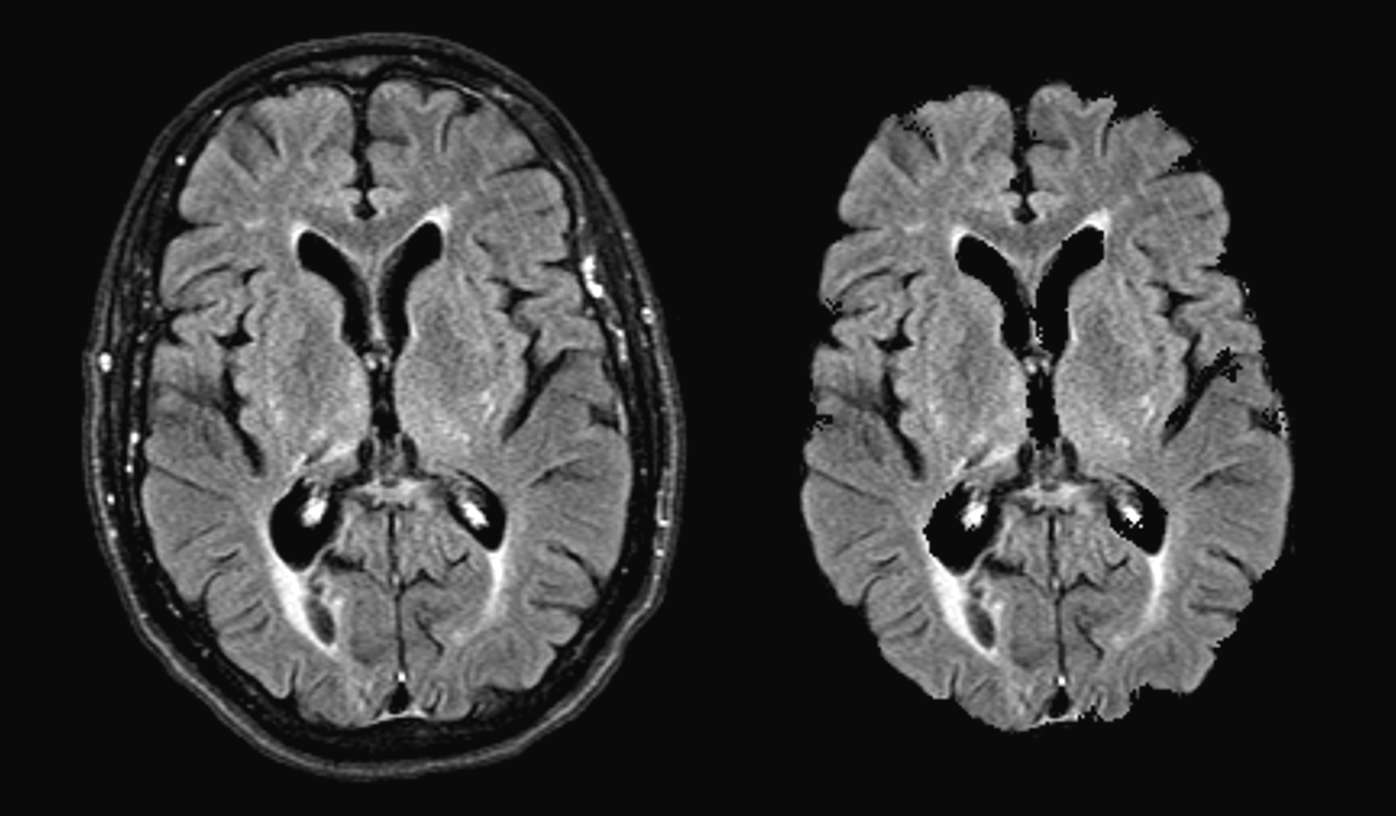
\includegraphics[width=7cm]{res.png}
\caption{Left: Program Input, Right: Program Output}
\end{figure}

\section{EVALUATION / CONCLUSION / RESULTS}
Overall, our results were very good. We were able to successfully use machine learning to skull strip axial MRIs of the brain. To evaluate our the performance of our solution, we computed the Dice score of each test image and averaged them. We achieved a mean Dice score of 97.02 using the two phased postprocessing approach. To put this into perspective, the result attained by the cutting edge solution developed by Kleesiek et al has a mean Dice score of 95.19 for clinical data. However, it is important to note that our testing set was very small (only 5 images) and so the uncertainty of this score is quite high. This was because the data we collected had a lot of tilted and shaken MRIs, some had large variations in sizes (which we avoided), and many were not coregistered. The final set of usable data was quite small. Our training set was also small and contained 13 images which were split into 2 sets for the two phased postprocessing. As we have seen in testing our program, more data usually improves our results and so we can expect additional data to increase our mean Dice score.

\section{DISCUSSION AND FUTURE WORK}
In the process of developing this tool we learned a lot about different classifiers and machine learning techniques. Although we are happy with our results, we believe that there is still lots of room for improvement. Since our data set was quite limited, we believe that we should collect more data to further improve our results. This extra data will also allow us to ensure that our algorithm works for data sets with higher ventricle and skull size variability. Furthermore, we should look into a more customized machine learning approach for postprocessing our output bit mask instead of using the same algorithm we are using to train the skull stripping.

\section*{ACKNOWLEDGMENT}

Thanks to the Dr. Fabien Scalzo for teaching us about magnetic resonance imaging and machine learning and UCLA for providing us with data to use for training and testing.

\begin{thebibliography}{99}

\bibitem{c1} Roy S, Maji P. A simple skull stripping algorithm for brain MRI. Eighth International Conference on Advances in Pattern Recognition (ICAPR). 2015;10.1109.
\bibitem{c2} Kleesiek J, Urban G, Hubert A, Schwarz D, Maier-Hein K, Bendszus M, Biller A. Deep MRI brain extraction: A 3D convolutional neural network for skull stripping. NeuroImage. 2016;129:460-469.

\end{thebibliography}

\end{document}
